\subsection{Validazione e collaudo}
	\subsubsection{Prospetto orario}
	La distribuzione oraria della fase di Validazione e collaudo è la seguente:
	
	\begin{table}[!htpb]
		\centering
		\renewcommand{\arraystretch}{2} 
		\rowcolors{2}{gray!25}{white}
		\begin{tabular}{|l c c c c c c|c| }
			\rowcolor{orange!50}
			\hline
			\multicolumn{8}{|c|}{\textbf{Suddivisione delle ore nei vari ruoli}}\\
			\hline
			\textbf{Nominativo} & RES 	& AMM 	& ANA 	& PRO 	& PRG 	& VER 	& \textbf{Totale} \\
			\hline
			\mat  				&-		& 12	&-		&-		&-		& 9		&21 \\
			\hline
			\pie  				&-		& 12	&-		&-		&-		& 9		&21\\
			\hline
			\mic  				&-		&-		&-		&-		& 6		& 15	&21\\
			\hline
			\mar  				&-		&-		&-		&-		& 10	& 11	&21\\
			\hline
			\daG  				& 8		&-		&-		&-		&-		& 13	&21\\
			\hline
			\daL  				&-		&-		&-		&-		&-		& 21	&21\\
			\hline
			\gia  				& 8		&-		&-		&-		&-		& 13	&21\\
			\hline
		\end{tabular}
		\caption{Suddivisione ore del periodo di Validazione e collaudo}
	\end{table}
	~\newline
	Di seguito rappresentata anche in un grafico:
\begin{figure}[!htpb]
	\centering
	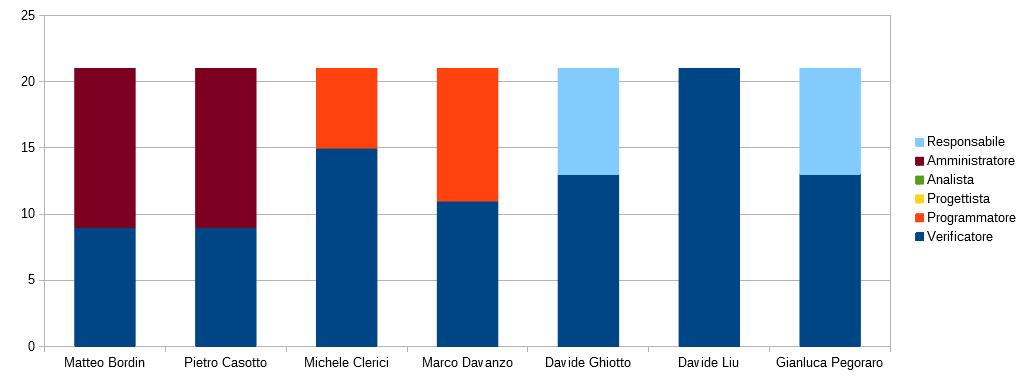
\includegraphics[width=\textwidth]{preventivo/grafico_quarta_parte.jpg}
	\caption{Grafico suddivisione oraria nel periodo di Validazione e collaudo}
\end{figure}
	\newpage
	\subsubsection{Conteggio ore}
	La distribuzione delle ore nei vari ruoli nella fase di Validazione e collaudo è la seguente:
	
	\begin{table}[!htpb]
			\centering
		\renewcommand{\arraystretch}{1.8} 
		\rowcolors{2}{gray!25}{white}
		\begin{tabular}{| c c c|}
			\rowcolor{orange!50}
			\hline
			\multicolumn{3}{|c|}{\textbf{Suddivisione delle ore nei vari ruoli}}\\
			\hline
			\textbf{Ruolo} 			& Ore 	& Costo\\
			\hline
			\textbf{Responsabile}	&16		&480\\
			\hline
			\textbf{Amministratore}	&24		&480\\
			\hline
			\textbf{Analista}		&0		&0\\
			\hline
			\textbf{Progettista}	&0		&0\\
			\hline
			\textbf{Programmatore}	&16		&240\\
			\hline
			\textbf{Verificatore} 	&91		&1365\\
			\hline
			\textbf{Totale} 		&147	&2565\\
			\hline 
		\end{tabular}
		\caption{Ore e costi totali del periodo di Validazione e collaudo}
	\end{table}
	~\newline Di seguito rappresentata anche in un grafico:
\begin{figure}[!htpb]
	\centering
	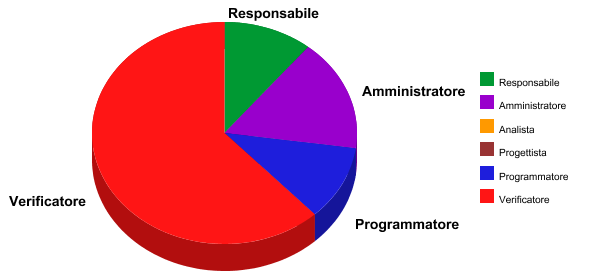
\includegraphics[scale=0.8]{preventivo/torta_quarta_parte.png}
	\caption{Grafico suddivisione ruoli nel periodo di Validazione e collaudos}
\end{figure}
\clearpage
